\subsection{Bayesian Linear Regression}\label{ssec:regression}

\begin{figure*}[t]
    \centering
    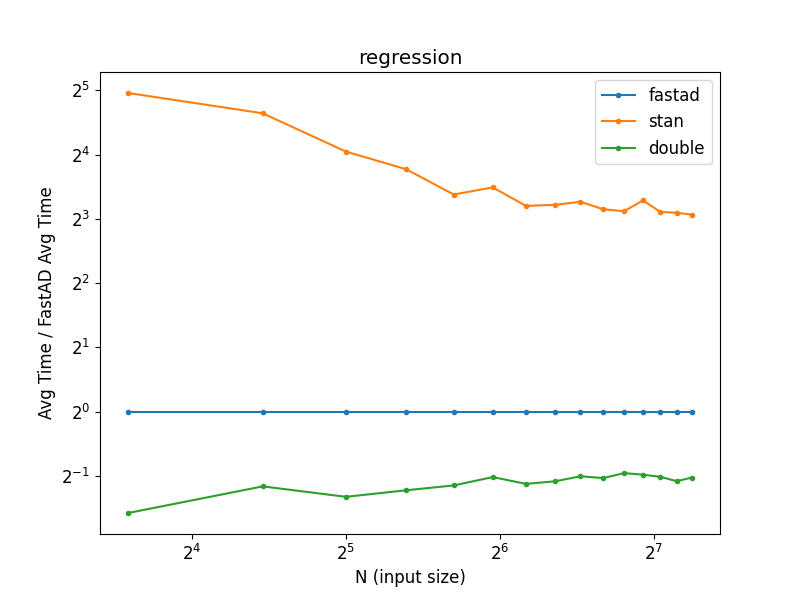
\includegraphics[width=0.75\textwidth]{figs/regression_fig.png}
    \caption{%
        Bayesian linear regression benchmark of Stan against FastAD 
        plotted relative to FastAD average time.
    }\label{fig:regression}
\end{figure*}

This section marks the first macro-benchmark example.
We consider the following Bayesian linear regression model:
\begin{align*}
    y &\sim N\paren{X\cdot w + b, \sigma^2} \\
    w &\sim N\paren{0,1} \\
    b &\sim N\paren{0,1} \\
    \sigma &\sim Unif\paren{0.1, 10.}
\end{align*}
The target function is the log of the joint probability density function (up to a constant).
Fig.~\ref{fig:regression} shows the benchmark results.

FastAD outperforms Stan by $ 8.6$ times for the largest $N$ and Adept by $ 10$ times.
The trend stabilizes starting from around $N=70$.
It is interesting to see that around $N=2^7$, 
FastAD is only $ 2.2$ times slower than the baseline,
despite the model consisting of a large matrix multiplication and many normal log-pdfs.
One of the reasons is that the compiler was able to optimize-out the backward-evaluation 
of the matrix constant $X$, since constants implement a no-op for backward-evaluation.

If we assume that the most expensive operation is the matrix multiplication,
AD evaluation approximately takes two matrix multiplications between a matrix and a vector.
We can then approximate a lower bound for the manually-written gradient computation time to be two times that of the baseline.
The relative time of FastAD to this approximated time is
$1.1$, implying about $ 10\%$ overhead from a manually-written code.
